\documentclass[a4paper, 11pt]{article}
\usepackage{graphicx}
\usepackage{amsmath}
\usepackage[pdftex]{hyperref}

% Lengths and indenting
\setlength{\textwidth}{16.5cm}
\setlength{\marginparwidth}{1.5cm}
\setlength{\parindent}{0cm}
\setlength{\parskip}{0.15cm}
\setlength{\textheight}{22cm}
\setlength{\oddsidemargin}{0cm}
\setlength{\evensidemargin}{\oddsidemargin}
\setlength{\topmargin}{0cm}
\setlength{\headheight}{0cm}
\setlength{\headsep}{0cm}

\renewcommand{\familydefault}{\sfdefault}

\title{Introduction to Learning and Intelligent Systems - Spring 2015}
\author{jo@student.ethz.ch\\ sakhadov@student.ethz.ch\\  stegeran@student.ethz.ch\\}
\date{\today}

\begin{document}
\maketitle

\section{Project 3 : Image Classification}

\subsection{ANN}
In a first attempt we used neural networks as feature learners combined with a logistic regression classifier. The scikit-learn package includes the restricted bolzmann machines (RBM) for unsupervised non-linear feature learners. To benchmark the learned features we first used logistic regression alone which gave us a error rate of 0.25. After grid searching one and two layers of pipelined RBMs together with the logistic regression classifier we always obtained a higher rate of wrong recognised samples compared to the direct usage of the classifier.

Because sklearn offers only one hidden layer, we tried out OpenCV because it allows to define an arbitrary amount of hidden layers. However OpenCV surprised us with its slowness. Also we found out that additional hidden layers (e.g. 1500, 1000, 200) did not make the score better, albeit using much more processing power.

We then used another neural network library (https://github.com/IssamLaradji/NeuralNetworks) which allowed us to reach a score of about 0.21 using one hidden layer with 500 neurons. However, after countless long grid searches and experiments, we were unable to make the score any better.

After initial experiments with Theano (a Python GPU computing library), we turned to the Lasagne Python NN Library. It allows to run ANNs very efficiently and is also very feature-rich, e.g. offering dropout layers. This way, we ran a deep multi-layer network containing 2048, 3048, 1000 and 200 layers with two dropout layers placed in between. This allowed us to reach our final score.


\subsection{PCA}

PCA could not extract the most prominent vectors of X. We concluded that the data is not linearly separable.

\subsection{Kernelized PCA}

We tried different kernels for PCA. Unfortunately the method was using too much memory and could not be executed at a reasonable time. Nevertheless we could extract the 1024 eigenvectors using sigmoid kernel. We then ran an SVM classifier with linear as well as with a non-linear kernel. However, this could not help us to achieve a better result. Figure \ref{fig:kPCA} depicts the decomposition level that could be achieved with PCA using sigmoid kernel.

%-------------------------------------------------- 
\begin{figure}[h]
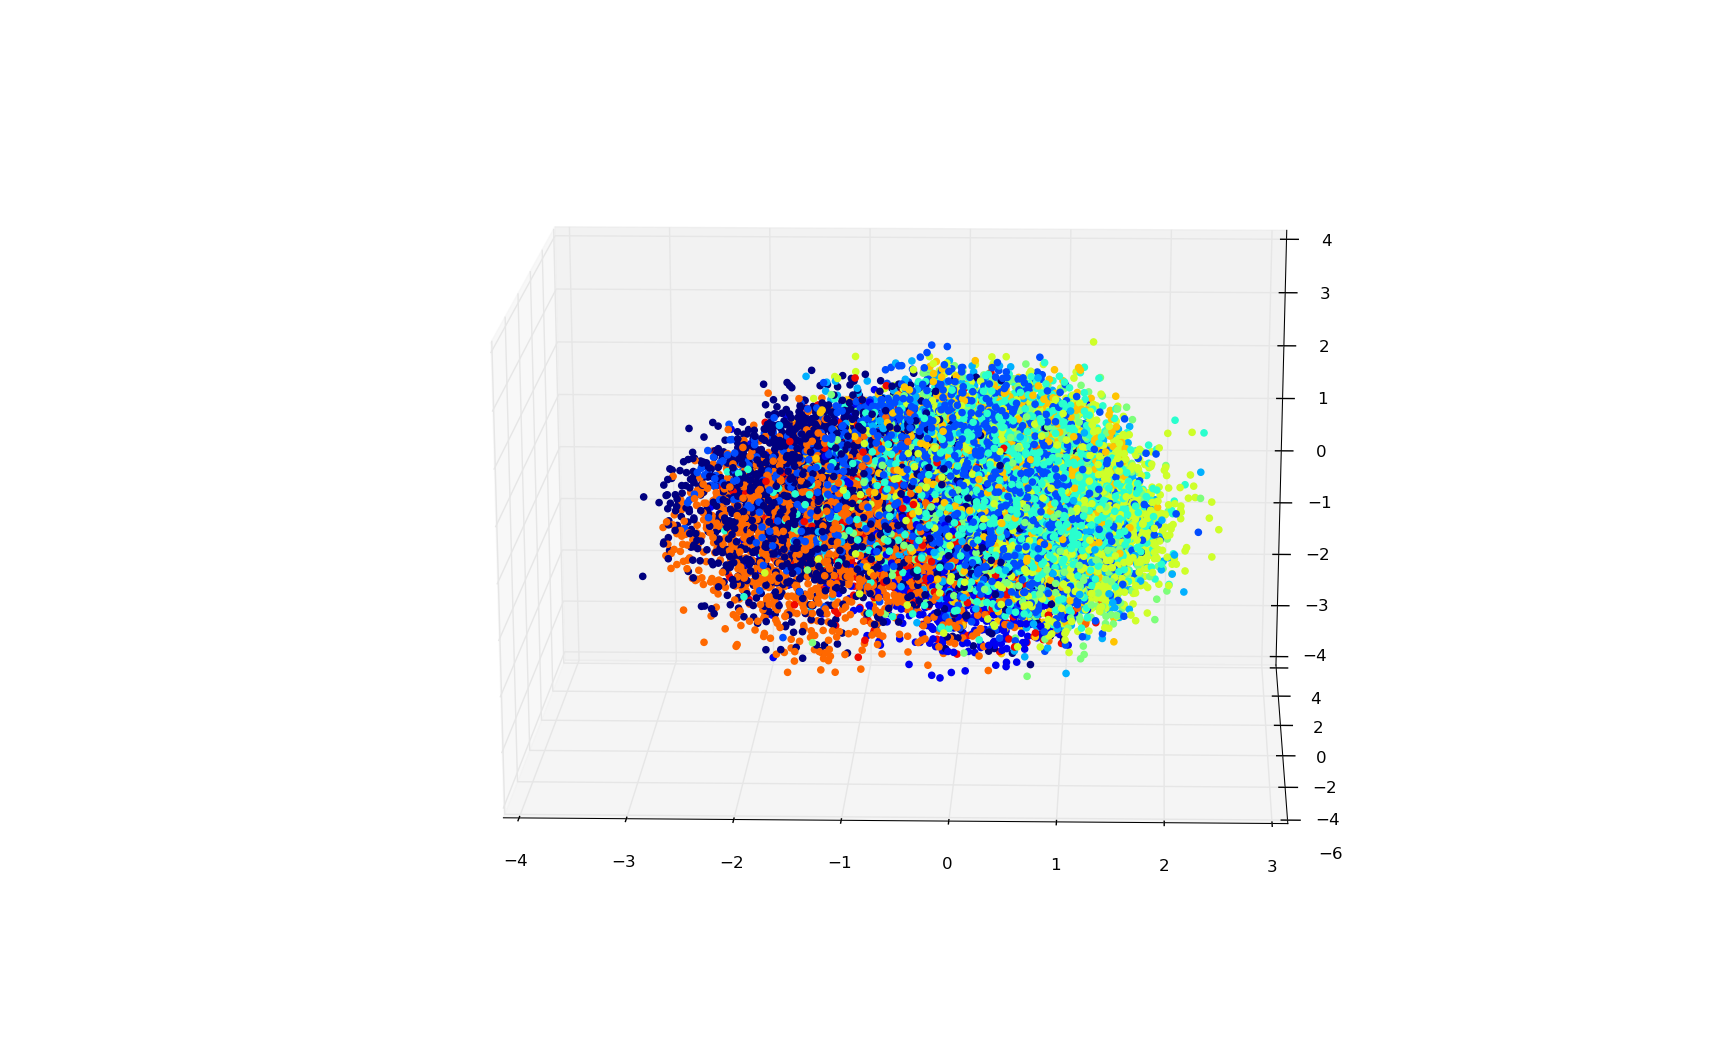
\includegraphics[width=0.9\linewidth]{img/kPCA.png} 
\caption{Classes data projected on the three greatest eigenvectors obtained through kernel PCA} 
\label{fig:kPCA}
\end{figure}




\subsection{Random Trees}

We tried to run random trees with different number of estimators. This, however did not bring us below our best result with neural networks.

\subsection{SVM}
We tried different kernels with SVM classifiers. The best result was achieved using the radial basis function kernel. 

\end{document}
